\documentclass[]{article}

\usepackage[utf8]{inputenc}
\usepackage{amsmath}
\usepackage{amssymb}
\usepackage{amsthm}
\usepackage{amsfonts}
\usepackage{graphicx}
\usepackage{capt-of}
\usepackage{listings}
\usepackage{siunitx}
\usepackage[section]{placeins}
\usepackage{float}



% Oppgavenummerering %
\renewcommand\thesection{Problem \arabic{section}}
\renewcommand\thesubsection{\alph{subsection})}

% Bevis
\newcommand\TombStone{\rule{.5em}{.5em}}
\renewcommand\qedsymbol{\TombStone}
\renewcommand{\proofname}{Bevis.} % Norske bevis

\title{TTK4215 – Assignment 10}
\author{Sigurd Totland | MTTK}

\begin{document}
\maketitle

\section{}
\subsection{}
To estimate the unknown $\xi$, We rewrite the system to be able to parametrize it,
\begin{equation}\begin{aligned}
(s^2 + 2\xi \omega_n s + \omega^2_n)y = \omega^2_n u \\
s \xi \omega_n sy =\omega^2_n u - s^2y - \omega^2_ny = \omega^2_n (u-y) - s^2y\\
\xi sy = \frac{1}{2}(\omega_n (u-y) - \frac{s^2y}{\omega_n}).
\end{aligned}\end{equation}
With this, we have only known signals on the left hand side, and a product of an unknown parameter and a known signal on the right hand side, just like we want. To make the system realizable however, we must ensure that the fractions are proper, so we filter both sides with a stable Hurwitz polynomial
\begin{equation}\begin{aligned}
\Lambda(s) = s^2 + \lambda_1 s + \lambda_0.
\end{aligned}\end{equation}
We then get
\begin{equation}\begin{aligned}
z = \frac{1}{2 \omega_n} \frac{\omega^2_n (u-y) - s^2y}{\Lambda} = \xi \frac{sy}{\Lambda} = \theta \phi.
\end{aligned}\end{equation}
We can then choose an estimation method of choice, such as gradient descent.

\subsection{}
We begin by assuming both parameters $\xi$ and $\omega_n$ known, and design an PPC scheme with the constant reference $y_m(t) = c$. We define polynomials $Z$ and $R$ from
\begin{equation}\begin{aligned}
y = \frac{Z}{R}u,
\end{aligned}\end{equation}
i.e. $Z$ has degree zero and $R$ degree $n = 2$. Furthermore, we require the polynomial $Q$ to satisfy $Qy_m = 0$, meaning $Q = s$ (because $\dot y_m = 0$ for constant $y_m$). To obtain stable control that makes $y \rightarrow y_m$, we define the control law
\begin{equation}\begin{aligned}
Q(s) L(s) u = -P(s) y + M(s) y_m
\end{aligned}\end{equation}
which yields
\begin{equation}\begin{aligned}
y = \frac{Z M}{LQR + PZ} y_m
\end{aligned}\end{equation}
with characteristic polynomial
\begin{equation}\begin{aligned}
LQR + PZ = 0.
\end{aligned}\end{equation}
We want an $A^*$ such that
\begin{equation}\begin{aligned}
A^* = LQR + PZ,
\end{aligned}\end{equation}
i.e. the closed loop becomes
\begin{equation}\begin{aligned}
y = \frac{ZM}{A^*}y_m
\end{aligned}\end{equation}
and
\begin{equation}\begin{aligned}
u = \frac{RM}{A^*}y_m.
\end{aligned}\end{equation}
Recall that
\begin{equation}\begin{aligned}
Z = \omega^2_n, \quad \text{and} \quad R = s^2 + 2 \xi \omega_n s + \omega_n^2.
\end{aligned}\end{equation}
Note how this control scheme only changes the poles in contrast to MRC in which the zeros are also changed. We must choose $L$ and $P$ such that the wanted control performance is achieved. From I\&S we know that $A^*$ will have order $4$. Also, $L$ will have order $1$ and $P$ order $2$. We hence define
\begin{equation}\begin{aligned}
L = (s + \lambda_1^L), \quad \text{and} \quad P = (s + \lambda_1^P) (s + \lambda_2^P).
\end{aligned}\end{equation}
With that, $A^*$ can be written out as
\begin{equation}\begin{aligned}
\label{eq:A_star_really}
A^* &= (s + \lambda_1^L) s (s^2 + 2 \xi \omega_n s + \omega^2_n) + \omega^2_n (s + \lambda_1^P)(s + \lambda_2^P) \\
&= s^4 + 2 \xi \omega_n s^3 + \omega_n^2 s^2 + \lambda_1^L s^3 + 2 \lambda_1^L \xi \omega_n s^2 + \lambda_1^L \omega_n^2 s\\
&+ \omega_n^2 s^2 + \omega_n^2 \lambda_2^P s + \omega_n^2 \lambda_1^P s + \omega_n^2 \lambda_1^P \lambda_2^P\\
&= s^4 + (2 \xi \omega_n + \lambda_1^L)s^3 + (\omega_n^2 + 2 \lambda_1^L \xi \omega_n + \omega_n^2)s^2\\
&+ (\lambda_1^L \omega_n^2 + \omega_n^2 \lambda_2^P + \omega_n^2 \lambda_1^P)s + \omega_n^2 \lambda_1^P \lambda_2^P.
\end{aligned}\end{equation}
To achieve the wanted controller performance of no more than $5\%$ overshoot and settling time $t_s$ less than 2 seconds, we must set some requirements on $A^*$. However, since $A^*$ is of order 4, we cannot formulate analytical expressions for these criteria. We can however do a sneaky trick which will yield acceptable results. We can view $A^*$ as the concatination of three systems, one of order 2 that we will do analysis on, and two first order systems that are much faster, and hence neglectable. $A^*$ as the system shown in figure \ref{fig:sys}.
\begin{figure}[H]
\centering
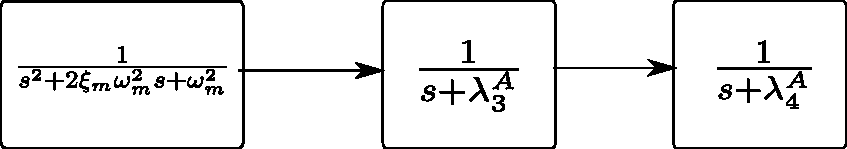
\includegraphics[width=0.6\textwidth]{system}
\caption{$A^*$ system}
\label{fig:sys}
\end{figure}
The first, second order system is the one we are the most interested in,
\begin{equation}\begin{aligned}
\frac{1}{(s + \lambda_1^A)(s + \lambda_2^A)} =
\frac{1}{s^2 + 2 \xi_m \omega_m + \omega^2_m}.
\end{aligned}\end{equation}
We can then match the wanted $A^*$ with the $A^*$ we have defined, i.e.
\begin{equation}\begin{aligned}
\label{eq:A_star_hell}
A^* &= s^4 + (\lambda_1^A + \lambda_2^A + \lambda_3^A + \lambda_4^A)s^3 \\
&+ (\lambda_3^A\lambda_4^A + \lambda_1^A\lambda_2^A + \lambda_1^A\lambda_3^A + \lambda_1^A\lambda_3^A + \lambda_2^A\lambda_3^A + \lambda_2^A\lambda_3^A + \lambda_2^A\lambda_4^A)s^2\\
&+ (\lambda_1^A\lambda_2^A\lambda_3^A + \lambda_1^A\lambda_2^A\lambda_4^A
+ \lambda_3^A\lambda_4^A\lambda_1^A + \lambda_3^A\lambda_4^A\lambda_2^A)s + \lambda_1^A\lambda_2^A\lambda_3^A\lambda_4^A
\end{aligned}\end{equation}
With the matched polynomials, we then require the two following criteria. Firstly, to ensure the overshoot is never any higher than $5\%$, we require (from Balchen et.al)
\begin{equation}\begin{aligned}
&1 + e^{-\frac{\xi_m}{\sqrt{1-\xi^2_m}}\pi} < 1.05\\
&\implies e^{-\frac{\xi_m}{\sqrt{1-\xi^2_m}}\pi} < 0.05\\
&\implies -\frac{\xi_m}{\sqrt{1-\xi^2_m}}\pi < \ln(0.05)\\
&\implies \xi_m \pi < \ln(0.05) \sqrt{1-\xi^2_m} \\
&\implies \xi_m^2 \pi^2 < \ln^2(0.05)(1 - \xi^2_m) \\
&\implies \xi_m^2 (\pi^2 + \ln^2(0.05)) < \ln^2(0.05) \\
\end{aligned}\end{equation}
which yields the requirement
\begin{equation}\begin{aligned}
\xi_m = \sqrt{\frac{\ln^2(0.05)}{\pi^2 + \ln^2(0.05)}}.
\end{aligned}\end{equation}
Secondly, for the settle time to be less than 2 seconds, we require
\begin{equation}\begin{aligned}
\frac{3.2}{\xi_m \omega_m} < 2
\end{aligned}\end{equation}
i.e.
\begin{equation}\begin{aligned}
\omega_m > \frac{1.6}{\xi_m}.
\end{aligned}\end{equation}
We also require the remaining poles, $\lambda_3^A$ and $\lambda_4^A$ to be sufficiently faster (further from zero) than $\lambda_1^A$ and $\lambda_2^A$. With these constraints, we can match the terms with same ordered $s$-terms in \eqref{eq:A_star_really} and \eqref{eq:A_star_hell} to finally solve for $L$ and $P$. Since $\xi$ is unknown, we must use the estimate calculated from the adaptive law in task a).

\section{I\&S 7.5}
\subsection{}
We have
\begin{equation}\begin{aligned}
y = \frac{s+b}{s(s+a)}u
\end{aligned}\end{equation}
which yields
\begin{equation}\begin{aligned}
sy(s+1) &= (s+b) u \\
s^2 y + sya &= su + ub \\
s^2y - su &= - sya + ub =
\begin{bmatrix} a & b \end{bmatrix}
\begin{bmatrix} -sy \\ u \\ \end{bmatrix}.
\end{aligned}\end{equation}
To realize an adaptive law based on this, we need both sides to be realizable, so we filter with a second order stable Hurwitz polynomial
\begin{equation}\begin{aligned}
\Lambda(s) = s^2 + \lambda_1 s + \lambda_0
\end{aligned}\end{equation}
and obtain
\begin{equation}\begin{aligned}
\frac{s^2 - su}{\Lambda} =
\begin{bmatrix} a & b \end{bmatrix}
\begin{bmatrix} \frac{-sy}{\Lambda} \\ \frac{u}{\Lambda} \\ \end{bmatrix},
\end{aligned}\end{equation}
i.e. we have $z = \theta^{*\top} \phi$ with
\begin{equation}\begin{aligned}
z = \frac{s^2 - su}{\Lambda}, \quad
\theta^{*\top} =
\begin{bmatrix} a & b \end{bmatrix}, \quad \text{and} \quad
\phi =
\begin{bmatrix} \frac{-sy}{\Lambda} \\ \frac{u}{\Lambda} \\ \end{bmatrix}.
\end{aligned}\end{equation}
This scheme can be combined with e.g. gradient descent to find estimates $\hat a$ and $\hat b$.

\subsection{}
We define
\begin{equation}\begin{aligned}
y = \frac{Z}{R},
\end{aligned}\end{equation}
where $> = s+b$ and $R = s(s+a)$. We note that de degree of $Z$ is one and the degree of $R$ is two. To regulate $y \rightarrow y_m = 0$, we define the control input $u$ by
\begin{equation}\begin{aligned}
QLu = -Py + My_m.
\end{aligned}\end{equation}
From this, we require
\begin{equation}\begin{aligned}
Qy_m = 0
\end{aligned}\end{equation}
and since $y_m = 0$, we can define $Q$ as we want, e.g. $Q=1$ for simplicity. This yields
\begin{equation}\begin{aligned}
Lu = -Py + My_m
\end{aligned}\end{equation}
which imlies
\begin{equation}\begin{aligned}
y = \frac{ZM}{LR + PZ}y_m.
\end{aligned}\end{equation}
The denominator in this expression we define as
\begin{equation}\begin{aligned}
A^* = LR + PZ.
\end{aligned}\end{equation}
The characteristic equation is then
\begin{equation}\begin{aligned}
A^* = LR + PZ = 0
\end{aligned}\end{equation}
We also note that $L$ and $P$ both have degree 1, so in total, $A^*$ has degree 3. We define the roots of $A^*$ (the poles of the closed loop system) as $p_1, p_2, \text{ and } p_3$ and get
\begin{equation}\begin{aligned}
A^* &= (s + p_1)(s+p_2)(s+p_3)\\
&= s^3 + s^2(p_1 + p_2 + p_3) + s(p_1 p_2 + p_1p_3 + p_2p_3) + p_1p_2p_3.
\end{aligned}\end{equation}
Furthermore, we write out the polynomials (defining $\lambda^L, \lambda^P$ as the roots of $L$ and $P$ respectively), obtaining
\begin{equation}\begin{aligned}
A^* &= LR + PZ \\
&= (s + \lambda^L)s(s+a) + (s+\lambda^P)(s+b) \\
&= s^3 + s^2(1 + \lambda^L + a) + s(\lambda^L a + \lambda^P + b) + \lambda^P b.
\end{aligned}\end{equation}
We then match the polynomials to find where we should place the roots of $A^*$ given parameters $a$ and $b$. This yields the equation set
\begin{equation}\begin{aligned}
p_1 + p_2 + p_3 &= 1 + \lambda^L + a \\
p_1 p_2 + p_1 p_3 + p_2 p_3 &= \lambda^L a + \lambda^P + b\\
p_1 p_2 p_3 &= \lambda"P b.
\end{aligned}\end{equation}
In order to solve this, we must of course know the values of the parameters $a$ and $b$, which we do not. To make an adaptive PPC scheme instead then, we replace $p_1, p_2$ and $p_3$ with estimates $\hat p_1(\hat a, \hat b)$, $\hat p_2(\hat a, \hat b)$, and $\hat p_3(\hat a, \hat b)$ and insert the on line estimates of $a$ and $b$ found in the previous subtask.

\subsection{}
When solving for $\lambda^P$ we might compute
\begin{equation}\begin{aligned}
\lambda^P = \frac{\hat p_1 \hat p_2 \hat p_3}{\hat b},
\end{aligned}\end{equation}
and must hence require that $\hat b \neq 0$. Likewize when we solve for $\lambda_L$, we might have to solve
\begin{equation}\begin{aligned}
\lambda^L = \frac{\hat p_1 \hat p_2 + \hat p_1 \hat p_3  + \hat p_2 \hat p_3 - \lambda^P + \hat b}{\hat a}
\end{aligned}\end{equation}
and hence $\hat a \neq 0$. We then usually require that $|\hat a| > 0$ and $|\hat b| > 0$ for all $t$.





\end{document}
